\subsection{Pengenalan Quartus Prime}

Quartus Prime merupakan perangkat lunak CAD (computer-assisted design)
yang digunakan untuk desain rangkaian digital. Quartus Prime dikembangkan
oleh Altera. Versi Lite dari Quartus Prime dapat diunduh secara gratis
pada laman Altera\footnote{\url{http://dl.altera.com/?edition=lite}}.
Quartus Prime dapat dijalankan pada
platform Windows dan Linux.
Jendela utama dari Quartus Prime Lite dapat dilihat pada Gambar
\ref{fig:main_window}.

\begin{figure}
\centering
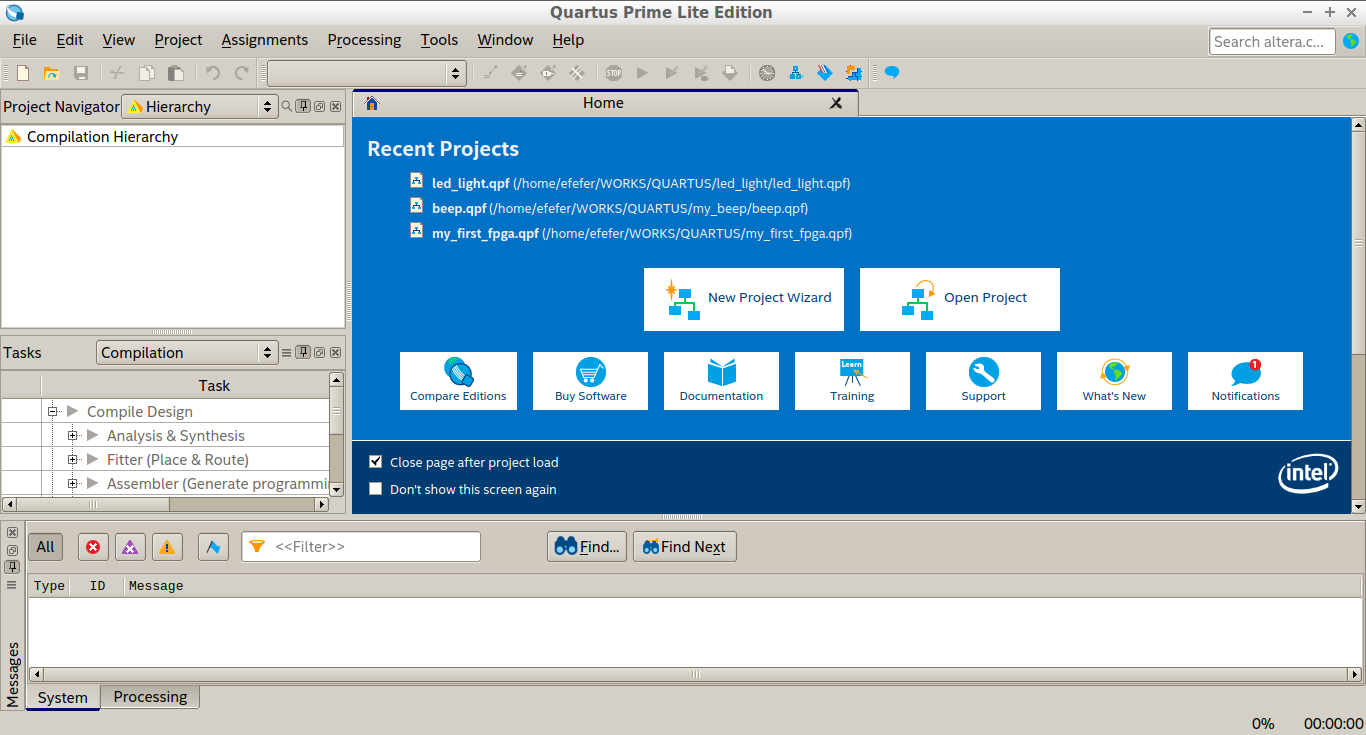
\includegraphics[width=\textwidth]{images/FirstOpen.png}
\par
\caption{Tampilan jendela utama Quartus Prime Lite}\label{fig:main_window}
\end{figure}

Dengan menggunakan CAD, setidaknya ada dua cara untuk
mendesain rangkaian digital:
\begin{itemize}
\item \textit{schematic capture}, dengan membuat skematik dari rangkaian yang
diinginkan.
\item menggunakan Hardware Description Language (HDL).
Dua jenis HDL yang paling populer adalah Verilog dan VHDL.
Kedua bahasa tersebut telah diadopsi sebagai IEEE Standard.
Pada tulisan ini akan digunakan Verilog.
\end{itemize}

Kita akan mulai dengan menggunakan skematik.

\subsection{Menambahkan skematik baru}

Skematik baru dapat ditambahkan ke dalam project dengan memilih menu
\textbf{File $\rightarrow$ New}. Pilih \textbf{New Diagram/Schematic File}, kemudian
\textbf{OK}.

\begin{figure}[H]
\centering
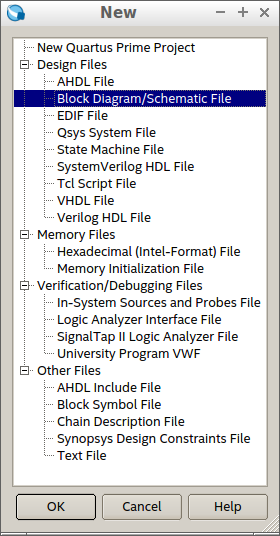
\includegraphics[scale=0.5]{images/NewSchematic.png}
\par
\end{figure}

File skematik kosong akan terbuka pada tab baru dengan nama \textbf{Block1.bdf}.
Kita dapat membuat skematik yang kita inginkan pada file ini.

\begin{figure}[H]
\centering
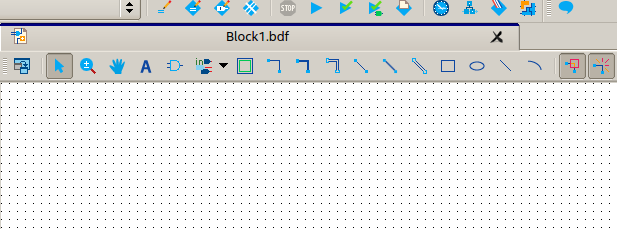
\includegraphics[scale=0.5]{images/EmptySchematic.png}
\par
\end{figure}

Untuk menambahkan komponen, dapat dilakukan dengan cara mengklik toolbar
\textbf{Symbol Tool}.

\begin{figure}[H]
\centering
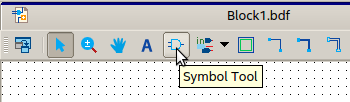
\includegraphics[scale=0.5]{images/SymbolTool.png}
\par
\end{figure}

Komponen yang ingin ditambahkan pada skematik dapat diperoleh dengan
ekspasi node \textbf{Libraries}, mencari komponen tersebut, dan memilihnya.
Misalkan kita ingin menambahkan gerbang AND dengan dua input, maka dapat dipilih
pada \textbf{primitives $\rightarrow$ logic $\rightarrow$ and2}. Klik
\textbf{OK} setelah komponen yang diinginkan telah dipilih.

\begin{figure}[H]
\centering
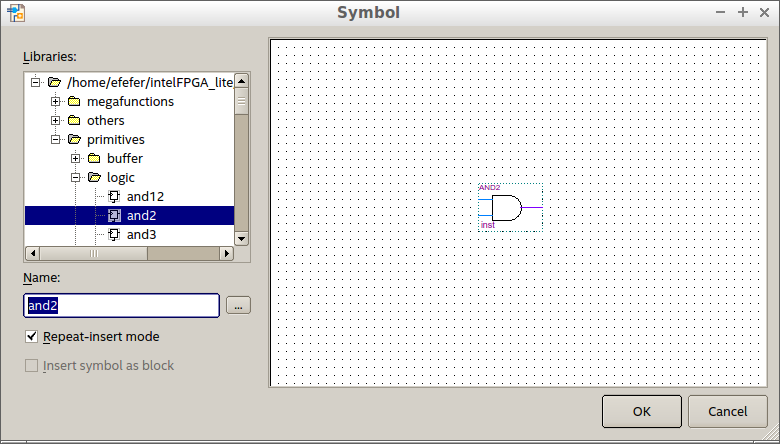
\includegraphics[scale=0.5]{images/BlockAnd.png}
\par
\end{figure}

Pemilihan komponen juga dapat dilakukan dengan mengetikkan nama komponen yang
diinginkan pada isian \textbf{Name}, misalnya \textbf{jkff} untuk J-K flip-flop.

Khusus untuk menambahkan komponen input dan output, dapat juga digunakan
toolbar \textbf{Pin Tool}.
\begin{figure}[H]
\centering
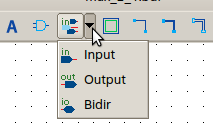
\includegraphics[scale=0.5]{images/PinTool.png}
\par
\end{figure}

Untuk menghubungkan antara satu komponen dengan komponen yang lain, dapat
digunakan \textbf{Orthogonal Node Tool}.
\begin{figure}[H]
\centering
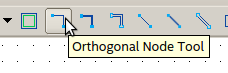
\includegraphics[scale=0.5]{images/OrthogonalNodeTool.png}
\par
\end{figure}

Berikut ini adalah contoh skematik untuk multiplexer 2-to-1:
\begin{figure}[H]
\centering
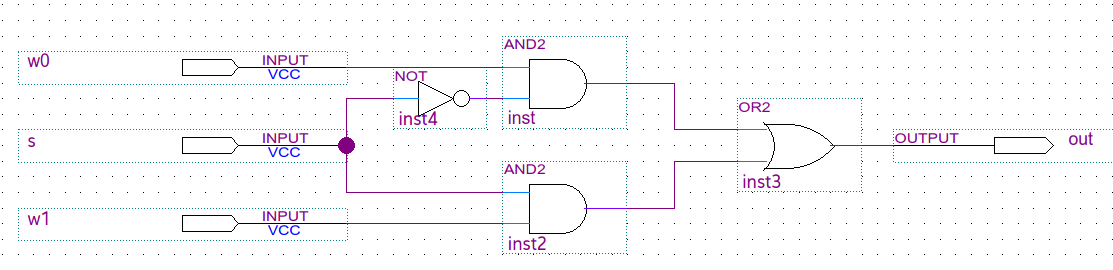
\includegraphics[width=\textwidth]{images/sch_mux_2_1.png}
\par
\end{figure}

Skematik ini kemudian dapat digunakan untuk proses lebih lanjut seperti
simulasi dan download ke hardware FPGA.

Menkonversi ke skematik ke simbol/blok sehingga dapat digunakan sebagai
bagian dari skematik lainnya: gunakan menu \textbf{File $\rightarrow$
Create/Update $\rightarrow$ Create Symbol Files for Current File}.

{\centering
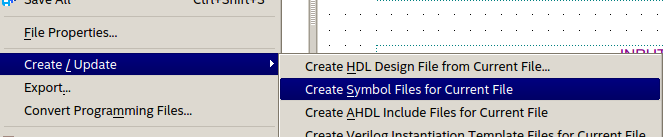
\includegraphics[scale=0.5]{images/MenuCreateSymbol.png}
\par}


